% !TeX spellcheck = de_DE
\documentclass[ngerman]{scrartcl} 

\KOMAoptions{fontsize=12pt, paper=a4}
\KOMAoptions{DIV=11}
\usepackage[utf8]{inputenc}             % Direkte Eingabe von ä usw.
\usepackage[T1]{fontenc}               	% Font Kodierung für die Ausgabe
\usepackage{babel}                   	% Verschiedenste sprach-spezifische Extras
\usepackage{parskip}
\usepackage[autostyle=true]{csquotes}	% Intelligente Anführungszeichen
\usepackage{amsmath}					% Mathematischer Formelsatz mit zusätzlichen mathematischen Schriften und Symbolen
\usepackage{amssymb}					% Mathematischer Formelsatz mit zusätzlichen mathematischen Schriften und Symbolen
\usepackage{physics}					% Differentialgleichungen
\usepackage{listings}					% Zum Einbinden von Programmcode verwenden wir das listings-Paket
\usepackage[dvipsnames]{xcolor}			% um Elemente von Befehlen farblich zu unterstützen
\usepackage[varg]{txfonts}              % Schönere Schriftart
\usepackage{graphicx}					% Paket um externe Graphiken einzufügen
\usepackage{media9}
\RequirePackage[backend=biber, style=numeric]{biblatex} % Literaturverzeichnis
\usepackage{hyperref} 					% um klickbare Elemente in Ihrem PDF-Ausgabedokument zu erzeugen
\RequirePackage[all]{hypcap} 			% ergänzend zu hyperref
\usepackage{siunitx}					% Intelligentes Setzten von Zahlen und Einheiten
\usepackage{enumitem}					% Aufzählungsarten
\usepackage{fancyhdr}
\usepackage{grffile}

\setlength\parindent{0pt} 				% Sets paragraph indentation to 0

\lstset{									% Deutsche Umlaute
	basicstyle=\ttfamily,    
	literate={~} {$\sim$}{1} 				% set tilde as a literal
	{ö}{{\"o}}1
	{ä}{{\"a}}1
	{ü}{{\"u}}1
	{ß}{{\ss}}1
	{Ö}{{\"O}}1
	{Ä}{{\"A}}1
	{Ü}{{\"U}}1
}

\lstset{
	numbers=left, 						% Line numbering
	numberstyle=\footnotesize, 			% Size of numbers
	basicstyle=\ttfamily\small, 		% Style and Size of Text
	backgroundcolor=\color{White}, 		% Background Color
	language=Python, 					% Language of Code
	commentstyle=\color{Maroon}, 		% Color and Style of Comments
	stringstyle=\color{OliveGreen}, 	% Color of Strings
	showstringspaces=false,
	morekeywords={import,from,class,def,for,while,if,is,in,elif,else,not,and,or,print,break,continue,return,True,False,None,access,as,del,except,exec,finally,global,import,lambda,pass,print,raise,try,assert}, 									% Definition of new keywords that will be highlighted
	keywordstyle=\color{RoyalBlue}		% Color and Style of Keywords
}


\pagestyle{fancy}
\fancyhf{}
\rhead{Ben Karcher, Anika Hoverath}
\lhead{Computerphysik - Abgabe 6}
\rfoot{Seite \thepage}

\title{Computerphysik - Abgabe 6}
\date{\today}


\begin{document}
	% Auf 3 setzen, da es beim ersten Chapter um 1 hochgezählt wird. 3+1=4
	\setcounter{section}{9}
	\thispagestyle{fancy}
	\renewcommand{\thesection}{H.\arabic{section}:}
	\renewcommand{\thesubsection}{H\arabic{section}.\arabic{subsection}}
	
\section{Schnelle \textsc{Fourier} Transformation (FFT) und Korrelationen}
In diesem Blatt betrachten wir die Anwendung des FFT algorithmus
um die Korrelation zweier Funktionen zu bestimmen.

\subsection{}

In diesem Aufgabenteil sollen die Gleichheiten:

\begin{equation}
\label{equ:1.3}
	[\mathcal{F}(f \odot g)]_{k} \underset{(1)}{=} [\mathcal{F} f]_{k}[\mathcal{F} g]_{-k} \underset{(2)}{=} [\mathcal{F} f]_{k} \overline{[\mathcal{F} \bar{g}]_{k}}
\end{equation}

gezeigt werden.

Dazu nutzen wir die Definition der \textsc{Fourier}-Transformation:

\begin{equation}
\label{equ:1.1}
	[\mathcal{F} f]_{k}=\sum_{j=0}^{N-1} f_{j} \exp (2 \pi i ~\frac{kj}{N})
\end{equation}

und den Ausdruck für die diskrete Korrelation für ein Zeitgitter der Länge $N$:

\begin{equation}
\label{equ:1.2}
	(f \odot g)_{k}:=\sum_{j=0}^{N-1} f_{j+k} g_{j}
\end{equation}

$\underline{\textbf{Zu (1):}}$\\
Für die erste Gleichheit setzen wir Gleichung \ref{equ:1.2} in Gleichung \ref{equ:1.1} ein und formen um:

\begin{align*}
	[\mathcal{F}(f \odot g)]_{k}
	&= \sum_{j=0}^{N-1} \left( \sum_{l=0}^{N-1} f_{l+j} g_{l} \right)  \exp (2 \pi i ~\frac{kj}{N})\\
	&= \sum_{l=0}^{N-1} g_l \sum_{j=0}^{N-1} f_{l+j} \exp (2 \pi i ~\frac{k(l+j-l)}{N})\\
	&= \sum_{l=0}^{N-1} g_l \underbrace{\sum_{j=0}^{N-1} f_{l+j} \exp (2 \pi i ~\frac{k(l+j)}{N})}_{[\mathcal{F} f]_{k}} \cdot \exp (2 \pi i ~\frac{-kl}{N})\\
	&= [\mathcal{F} f]_{k} \underbrace{\sum_{l=0}^{N-1} ~ g_l \cdot \exp (2 \pi i ~\frac{-kl}{N})}_{[\mathcal{F} g]_{-k}}\\
	&= [\mathcal{F} f]_{k} [\mathcal{F} g]_{-k}\\
\end{align*}





$\underline{\textbf{Zu (2):}}$\\
Es bleibt also zu zeigen:
\begin{equation*}
	[\mathcal{F} g]_{-k}= \overline{[\mathcal{F} \bar{g}]_{k}}
\end{equation*}

wir wissen, dass:
\begin{align*}
	[\mathcal{F} g]_{-k}= \sum_{l=0}^{N-1} ~ g_l \cdot \exp (2 \pi i ~\frac{-kl}{N})
\end{align*}
Außerdem:
\begin{align*}
[\mathcal{F} \overline{g}]_{-k}= \sum_{l=0}^{N-1} ~ \overline{g_l} \cdot \exp (2 \pi i ~\frac{kl}{N})
\end{align*}

Da für die komplexe Konjugation $\overline{y \cdot z}=\bar{y} \cdot \bar{z}$ gilt, lassen sich die beiden Faktoren einzeln komplex konjugieren, was dazu führt, dass $\overline{\overline{g_l}}=g_l$ ist und sich das Vorzeichen, des Terms ändert, der in der e-Funktion steht. Wir erhalten:
\begin{align*}
	\overline{[\mathcal{F} \bar{g}]_{k}}=\sum_{l=0}^{N-1} ~ g_l \cdot \exp (2 \pi i ~\frac{-kl}{N})
\end{align*}


Damit ist auch die zweite Gleichheit gezeigt und die Gleichung \ref{equ:1.3} kann genutzt werden.


\subsection{}
\label{ssec:10.2}

Zunächst soll hier $e(t)=s\left(t-t_{L}\right)+r(t)+b \sin (2 \pi \beta t)$ berechnet werden. Die Implementation dazu ist in \emph{main.cpp} zu finden. Um die Zufallszahlen zu generieren haben wir die \verb|C|-eigene \verb|random|-Funktion genutzt.\\
Anschließend haben wir $|e(t)|^2$ für die Amplituden $a=b=0.5, 1.0, 2.0, 4.0, 8.0, 16.0$ geplottet (Abbildung \ref{fig:2.1}).

\begin{figure}[htbp]
	\centering
	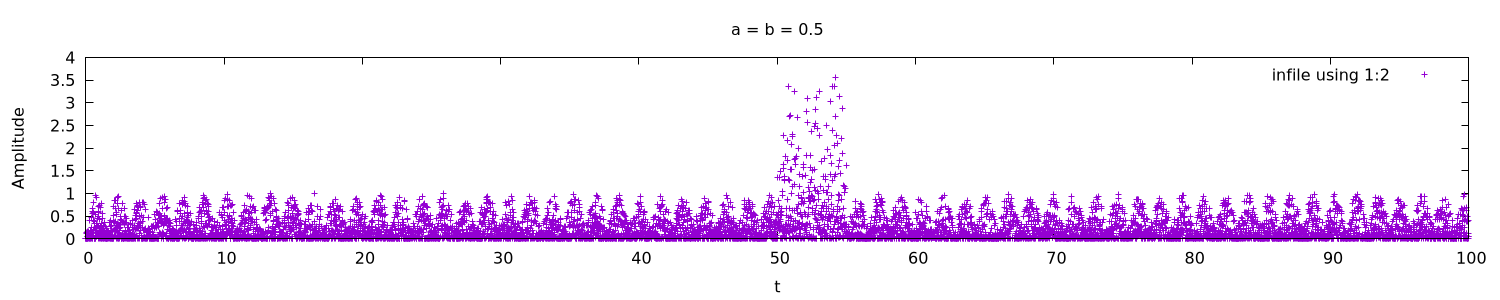
\includegraphics[width=0.98\textwidth]{plots/echo/0.5}
	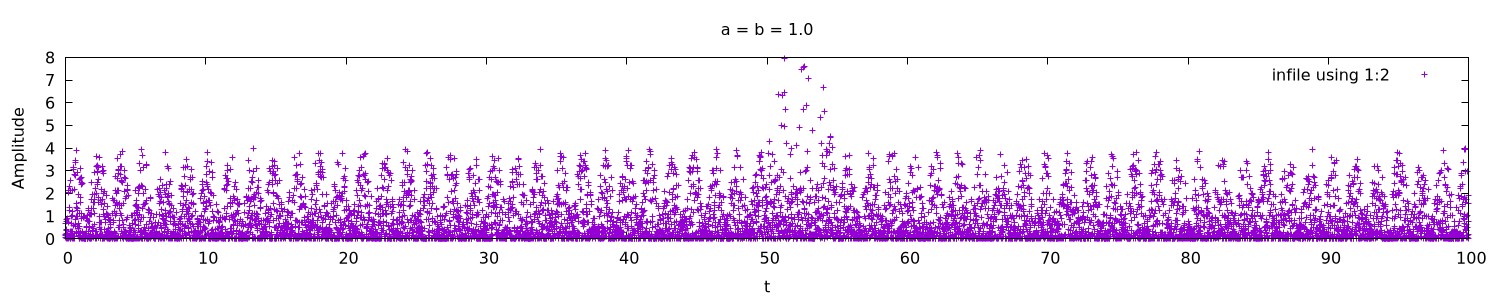
\includegraphics[width=0.98\textwidth]{plots/echo/1.0}
	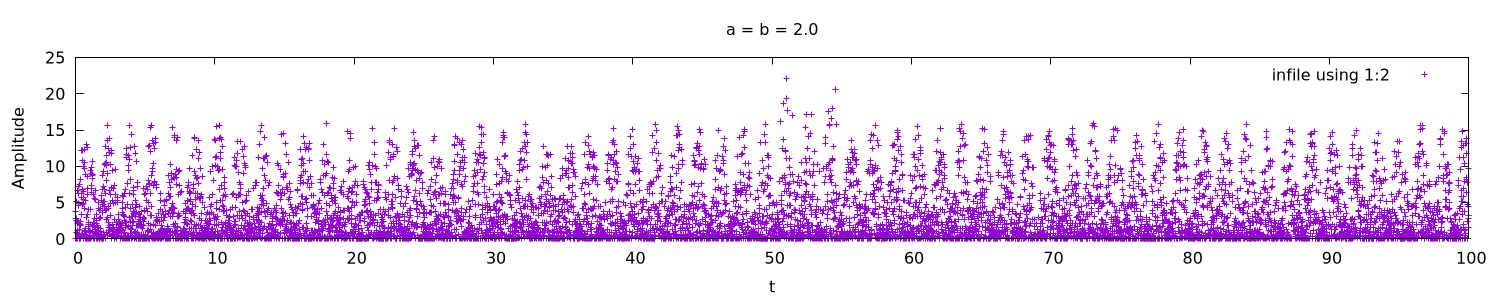
\includegraphics[width=0.98\textwidth]{plots/echo/2.0}
	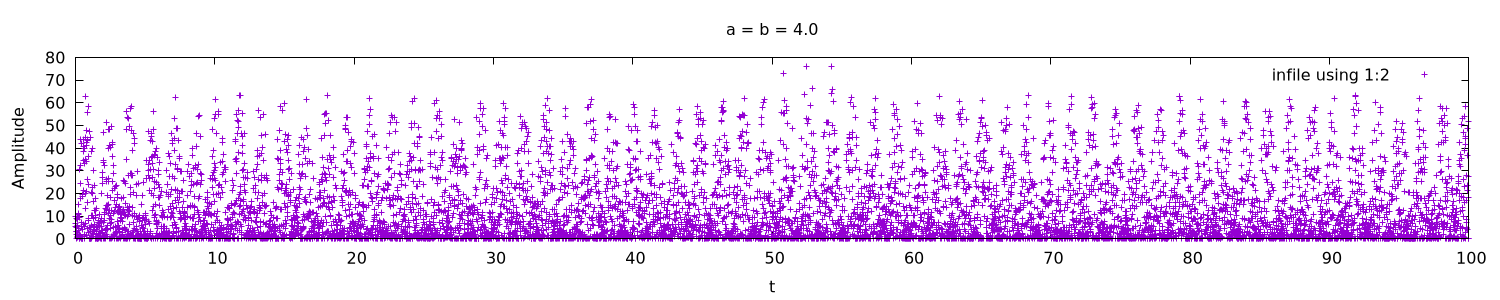
\includegraphics[width=0.98\textwidth]{plots/echo/4.0}
	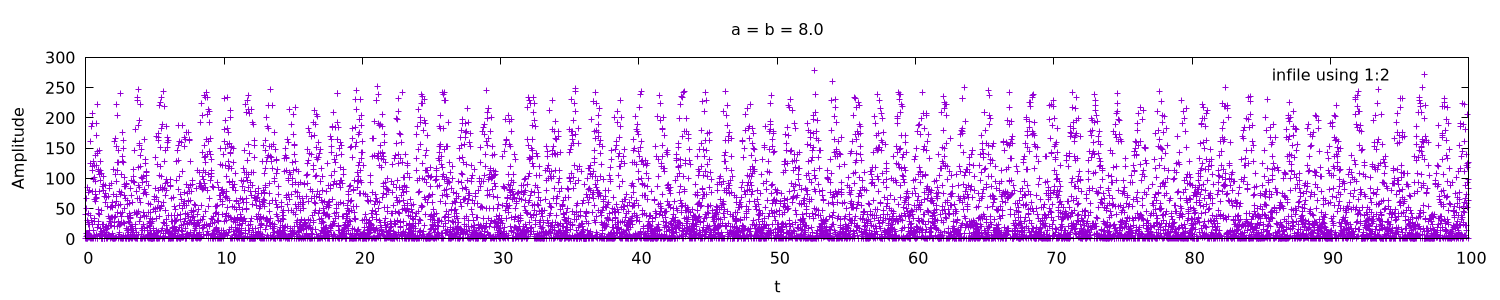
\includegraphics[width=0.98\textwidth]{plots/echo/8.0}
	\caption[$|e(t)|^2$]{Hier ist $|e(t)|^2$ für die Amplituden $a=b=0.5, 1.0, 2.0, 4.0, 8.0, 16.0$ dargestellt.}
	\label{fig:2.1}
\end{figure} 


Es lässt sich erkennen, dass für die Amplituden $a=b=0.5, 1.0, 2.0$ die Zeit $t_L$ noch sehr gut mit dem Auge abzulesen ist. Für $a=b=4$ ist es schon schwer die erste Amplitude des Echo-Signals und damit $t_L$ genau zu identifizieren. Für die Werte $a=b=8.0, 16.0$ ist es quasi nicht mehr möglich das Signal zu erkennen und damit auch nicht möglich $t_L$ abzulesen. 




\subsection{}

In dieser Teilaufgabe soll die Korrelation $(e \odot s)_k$ mithilfe der Methode der schnellen \textsc{Fourier}-Transformation (FFT) bestimmt werden. Die Korrelation ist hierbei eine Möglichkeit um ein bekanntes Signal, welches sich in Rauschen (also einem gestörten Umgebungssignal) befindet zu identifizieren. Dafür wendet man die \textsc{Fourier}-Transformation doppelt an:

\begin{equation*}
	(e \odot s)_{k}=\left[\mathcal{F}^{-1}\left( [\mathcal{F} e] \overline{[\mathcal{F} s]}\right)\right]_{k}, \quad k=0, \ldots, N-1
\end{equation*}
.

Die Implementation für das gesamte Programm ist wiederum in \emph{main.cpp} zu finden. Die Routine, die die FFT durchführt ist selber in der Datei \emph{fft.hpp} zu finden, welche allerdings in \emph{main.cpp} als \verb|header|-Datei eingebunden ist.

Nun haben wir die Korrelation $|(e \odot s)(t)|^{2}$ für die gleichen Störungsamplituden wie in Aufgabe \ref{ssec:10.2} berechnet ($a=b=0.5,1.0 2.0, 4.0, 8.0, 16.0$) und dargestellt (Abbildung \ref{fig:3.1}).

% \begin{figure}[htbp]
% 	\centering
% 	\includegraphics[width=0.98\textwidth]{figs/korrelation0.5}
% 	\includegraphics[width=0.98\textwidth]{figs/korrelation1}
% 	\includegraphics[width=0.98\textwidth]{figs/korrelation2}
% 	\includegraphics[width=0.98\textwidth]{figs/korrelation4}
% 	\includegraphics[width=0.98\textwidth]{figs/korrelation8}
% 	\includegraphics[width=0.98\textwidth]{figs/korrelation16}
% 	\caption[$|(e \odot s)(t)|^2$]{Hier ist die Korrelation $|(e \odot s)(t)|^2$ für die Amplituden $a=b=0.5, 1.0, 2.0, 4.0, 8.0, 16.0$ dargestellt.}
% 	\label{fig:3.1}
% \end{figure} 

Hier lässt sich nun erkennen, dass es wesentlich einfacher ist $t_L$ zu bestimmen, da man einfach nur den Zeitwert, an dem sich das Maximum der Funktion befindet, bestimmen muss. Dies funktioniert für die Störungsamplituden $a=b=0.5,1,2,4$ sehr gut. Bei höheren Störungsamplituden scheitert allerdings das verwendete Verfahren, wie man gut erkennen kann. Hier lässt sich der gesuchte Peak nicht mehr eindeutig identifizieren.






\subsection{}

Hier ist zu zeigen, dass das Ergebnis der Korrelation:
\begin{equation*}
	(e \odot s)(t):=\int_{-\infty}^{\infty} \mathrm{d} \tau~ e(t+\tau) s(\tau)
\end{equation*}
mit (da $a=b=0$)
\begin{equation}
\label{equ:5.1}
	e(t)= s(t-t_l)
\end{equation}

geschrieben werden kann als (wobei wir vier Intervalle unterscheiden):

\begin{itemize}
	\item [(1)] {$\mathbf{t<t_L-t_{max}}$}
	\begin{equation*}
		(e \odot s)(t)=0
	\end{equation*}
	\item [(2)] {$\mathbf{t_L-t_{max}<t<t_L}$}
	\begin{equation*}
		(e ~\odot~ s)(t)=\frac{1}{2} \cos \left(2 \pi \alpha\left(t-t_{L}\right)\right)\left(t_{\max }-t_{L}+t\right) -\frac{1}{4 \pi \alpha} \cos \left(2 \pi \alpha t_{\max }\right) \sin \left(2 \pi \alpha\left(t_{\max }-t_{L}+t\right)\right)
	\end{equation*}
	\item [(3)] {$\mathbf{t_L<t<t_L+t_{max}}$}
	\begin{equation*}
		(e ~\odot~ s)(t)= \frac{1}{2} \cos \left(2 \pi \alpha\left(t-t_{L}\right)\right)\left(t_{L}-t+t_{\max }\right) -\frac{1}{4 \pi \alpha} \cos \left(2 \pi \alpha t_{\max }\right) \sin \left(2 \pi \alpha\left(t_{\max }+t_{L}-t\right)\right)
	\end{equation*}
	\item [(4)] {$\mathbf{t_L+t_{max}<t}$}
	\begin{equation*}
		(e \odot s)(t)=0
	\end{equation*}
\end{itemize}


Es gilt nun allgemein:
\begin{equation}
\label{equ:5.2}
	s(\tau)=\left\{\begin{array}{ll}
	\sin (2 \pi \alpha \tau) & \text { für } 0 \leq \tau \leq t_{\max } \\
	0 & \text { sonst }
	\end{array}\right.
\end{equation}
.

$\underline{\textbf{Fall (1):}}$

In diesem Fall ergibt sich durch Einsetzen der Gleichung \ref{equ:5.1} in die Gleichung \ref{equ:5.2}:

\begin{equation*}
e(t+\tau)=\left\{\begin{array}{ll}
\sin (2 \pi \alpha (t+\tau-t_L)) & \text { für } 0 \leq t+\tau-t_L \leq t_{\max } \\
0 & \text { sonst }
\end{array}\right.
\end{equation*}
	
Da wir, um die Korrelation zu bestimmen, $s(\tau)$ mit $e(t+\tau)$ multiplizieren und es genügt, dass einer der Terme 0 ist müssen wir hier nur den Bereich betrachten, in dem $s(\tau)$ nicht 0 ist also $\tau \in [0,t_{max}]$.

Es wird der Bereich $t<t_L-t_{max}$ betrachtet, daraus folgt direkt das gilt: \\
$t+\tau-t_L< t_L -t_{max}+\tau -t_L=\tau-t_{max}$

Wenn man nun das $\dq$erlaubte$\dq$ ~Intervall von $\tau \in [0,t_{max}]$ betrachtet, kann man leicht erkennen, dass:
$\tau- t_{max} \leq 0$, womit auch $t+\tau-t_L \leq 0$ und damit ergibt $e(t+\tau)$ im Intervall $\tau \in [0,t_{max}]$ für die gegebene Bedingung $t<t_L-t_{max}$: 0. Insgesamt ist die Korrelation hier also 0, die gegebene Aussage (1) ist dementsprechend richtig.\\



$\underline{\textbf{Fall (2):}}$

Hier soll das Intervall $t_L-t_{max}<t<t_L$ betrachtet werden. $e(t+\tau)$ ist wieder:

\begin{equation*}
e(t+\tau)=\left\{\begin{array}{ll}
\sin (2 \pi \alpha (t+\tau-t_L)) & \text { für } 0 \leq t+\tau-t_L \leq t_{\max } \\
0 & \text { sonst }
\end{array}\right.
\end{equation*}

allerdings kann man die Intervallgrenzen umschreiben zu:

\begin{equation*}
e(t+\tau)=\left\{\begin{array}{ll}
\sin (2 \pi \alpha (t+\tau-t_L)) & \text { für } -t+t_L \leq \tau \leq t_{\max } -t+t_L \\
0 & \text { sonst }
\end{array}\right.
\end{equation*}


Wir haben also die Integralgrenzen $-t+t_L\leq \tau \leq t_{max}-t+t_L$ für $e(t+\tau)$, nun müssen wir noch überprüfen, ob sie mit den Grenzen von $s(\tau)$, in denen diese Funktion nicht 0 ergibt, übereinstimmen. Beim Einsetzen der Intervallgrenzen: $t_L-t_{max}<t<t_L$ in die untere Integralgrenze ergeben sich keine Verschiebungen, da dieses Intervall vollständig im $\dq$erlaubte$\dq$~ Intervall von $s(\tau)$ liegt. Beim Einsetzen der Intervallgrenzen in die obere Integralgrenze, zeigt sich jedoch, dass die Grenze bei $2 \cdot t_{max}$ anstatt bei $t_{max}$ liegt, sodass wir diese Integralgrenze auf $t_{max}$ verschieben müssen.\\
Nun können wir also das Integral aufstellen:
\begin{align*}
	(e ~\odot~ s)(t)=\int_{-t+t_L}^{t_{max}} \sin (2 \pi \alpha (t+\tau-t_L)) \cdot \sin (2 \pi \alpha \tau)~ d \tau
\end{align*}

Mithilfe des Additionstheorems $\sin \alpha \sin \beta = \frac{1}{2} \left[ \cos(\alpha-\beta) - \cos (\alpha+\beta) \right]$ lässt sich das Integral umschreiben zu:
\begin{align*}
(e ~\odot~ s)(t)=\int_{-t+t_L}^{t_{max}} \frac{1}{2} \left[ \cos(2 \pi \alpha (t-t_L)) - \cos (2\pi \alpha(t-t_L+2 \tau)) \right] ~ d \tau
\end{align*}

Dies lässt sich einfach lösen:

\begin{align*}
(e ~\odot~ s)(t)=\left[ \dfrac{\cos\left(2{\pi}a\left(t-t_L\right)\right)\tau}{2}-\dfrac{\sin\left(2{\pi}a\left(2\tau+t-t_L\right)\right)}{8{\pi}a} \right]_{-t+t_L}^{t_{max}}
\end{align*}

Mit Einsetzen der Grenzen und dem Additionstheorem $\sin \alpha +\sin \beta = 2 \sin \frac{\alpha + \beta}{2} \cos \frac{\alpha - \beta}{2}$ ergibt sich:

\begin{equation*}
	(e ~\odot~ s)(t)=\frac{1}{2} \cos \left(2 \pi \alpha\left(t-t_{L}\right)\right)\left(t_{\max }-t_{L}+t\right) -\frac{1}{4 \pi \alpha} \cos \left(2 \pi \alpha t_{\max }\right) \sin \left(2 \pi \alpha\left(t_{\max }-t_{L}+t\right)\right)
\end{equation*}

Der Zusammenhang (2) ist damit bestätigt.\\


$\underline{\textbf{Fall (3):}}$

Hier funktionieren die Überlegungen äquivalent zu Fall (2):

Durch das gegebene Intervall $t_L < t < t_L + t_{max}$ kann hier die obere Integralgrenze $t_{max}-t+t_L$ unverändert bleiben, die untere muss allerdings angepasst werden zu 0, da diese Grenze der Grenze des $\dq$erlaubten$\dq$~ Intervall von $s(\tau)$ entspricht. Hier ist also das Integral:

\begin{align*}
(e ~\odot~ s)(t)=\int_{0}^{t_{max}-t+t_L} \sin (2 \pi \alpha (t+\tau-t_L)) \cdot \sin (2 \pi \alpha \tau)~ d \tau
\end{align*}

zu lösen. Dies funktioniert genau wie in Fall (2), sodass wir die Rechnung hier nicht nochmal gesondert aufführen. Es ergibt sich:
\begin{equation*}
	(e ~\odot~ s)(t)= \frac{1}{2} \cos \left(2 \pi \alpha\left(t-t_{L}\right)\right)\left(t_{L}-t+t_{\max }\right) -\frac{1}{4 \pi \alpha} \cos \left(2 \pi \alpha t_{\max }\right) \sin \left(2 \pi \alpha\left(t_{\max }+t_{L}-t\right)\right)
\end{equation*}

Damit ist der Zusammenhang (3) bestätigt.\\


$\underline{\textbf{Fall (4):}}$

Die letzte Relation lässt sich sehr ähnlich zu Fall (1) belegen.


\begin{equation*}
e(t+\tau)=\left\{\begin{array}{ll}
\sin (2 \pi \alpha (t+\tau-t_L)) & \text { für } 0 \leq t+\tau-t_L \leq t_{\max } \\
0 & \text { sonst }
\end{array}\right.
\end{equation*}

Da wir, um die Korrelation zu bestimmen, $s(\tau)$ mit $e(t+\tau)$ multiplizieren und es genügt, dass jeweils einer der Terme 0 ist, müssen wir hier nur den Bereich betrachten, in dem $s(\tau)$ nicht 0 ist also $\tau \in [0,t_{max}]$.

Es wird der Bereich $t>t_L+t_{max}$ betrachtet, daraus folgt direkt das gilt: \\
$t+\tau-t_L>t_L+t_{max}+\tau-t_L=t_{max}+\tau$

Wenn man nun das $\dq$erlaubte$\dq$ ~Intervall von $\tau \in [0,t_{max}]$ betrachtet, kann man leicht erkennen, dass:
$t_{max}+\tau \geq t_{max}$, womit auch $t+\tau-t_L \geq t_{max}$ und damit ergibt $e(t+\tau)$ im Intervall $\tau \in [0,t_{max}]$ für die gegebene Bedingung $t>t_L+t_{max}$: 0. Insgesamt ist die Korrelation hier also 0, die gegebene Aussage (4) ist dementsprechend richtig.\\


Nachdem wir hier die gegebene Lösung der Korrelationen bewiesen haben, wollen wir diese analytische Lösung noch mit der numerisch bestimmten Lösung vergleichen, wobei wir keine Störung betrachten ($a=b=0$). Beide Graphen sind in das Diagramm \ref{fig:4.1} geplottet. Hierbei müssen wir für einen sinnvollen Vergleich allerdings den numerischen Wert noch mit dem Faktor $4,5 \cdot 10^7$ skalieren, damit die Maximalwerte übereinstimmen.

% \begin{figure}[htbp]
% 	\centering
% 	\includegraphics[width=0.98\textwidth]{figs/analKorrelation}
% 	\caption[Vergleich]{Hier haben wir die analytische (\textit{lila}) mit der numerischen(\textit{grün}) Lösung der Korrelation ohne Störung ($a=b=0$) verglichen.}
% 	\label{fig:4.1}
% \end{figure} 

Es lässt sich erkennen, dass die Einhüllende der analytischen und der numerischen Lösung sich sehr ähnlich sind, das numerische Verfahren hat also sehr gut funktioniert.

\subsection{}

In der letzten Aufgabe nutzen wir einen kleinen Trick um das bisher genutzte Verfahren zu besseren Ergebnissen zu führen. Wir versehen das gesendete Signal mit einem \emph{Zwitscher}-Puls, welcher eine bessere Autokorrelation aufweist. Das Signal wird dann beschrieben durch:
\begin{align*}
s(t)=\left\{\begin{array}{ll}
\sin (2 \pi (\alpha_0+\alpha_1 t) t)&,\text { für } 0 \leq t \leq t_{\max } \\
0& ,\text { sonst }
\end{array}\right.\\
\text{ mit } \alpha_0=5.0, \alpha_1=1.0
\end{align*}

Dieses Signal fügen wir dann in das schon erstellte Programm (\emph{main.cpp}) ein und plotten erneut die Korrelation $(e \odot s)(t)$ für die verschiedenen Störamplituden\\ $a=b=0.5, 1.0, 2.0, 4.0, 8.0, 16.0$ ; siehe Abbildung \ref{fig:5.1}.



% \begin{figure}[htbp]
% 	\centering
% 	\includegraphics[width=0.98\textwidth]{figs/korrelationB0.5}
% 	\includegraphics[width=0.98\textwidth]{figs/korrelationB1}
% 	\includegraphics[width=0.98\textwidth]{figs/korrelationB2}
% 	\includegraphics[width=0.98\textwidth]{figs/korrelationB4}
% 	\includegraphics[width=0.98\textwidth]{figs/korrelationB8}
% 	\includegraphics[width=0.98\textwidth]{figs/korrelationB16}
% 	\caption[$|(e \odot s)(t)|^2$]{Hier ist die Korrelation $|(e \odot s)(t)|^2$ für ein Zwitscher-Signal für die Störamplituden $a=b=0.5, 1.0, 2.0, 4.0, 8.0, 16.0$ dargestellt.}
% 	\label{fig:5.1}
% \end{figure} 


Das \emph{Zwitscher}-Signal hat das Verfahren tatsächlich effektiver gemacht. Nun lässt sich nämlich bis zu einer Störamplitude $a=b=8$ der Zeitwert $t_L$ genau bestimmen. Lediglich für $a=b=16$ ergibt sich kein sinnvolles Ergebnis mehr.


\end{document}

